\documentclass{article}
\title{Region layering}
\author{}
\date{}

\usepackage{graphicx,amsmath}
\begin{document}
\maketitle

\section{Introduction}

When regions overlap in time, we need to decide which one should be
played.


\section{Layers}

Each region on a playlist is on a \emph{layer}.  All overlapping regions
are on a unique layer, and when overlaps exist the highest-layered
region is played.  This is illustrated in Figure~\ref{fig:basic-layering}.

\begin{figure}[ht]
\begin{center}
\includegraphics{basic-layering.pdf}
\end{center}
\caption{Basic region layering}
\label{fig:basic-layering}
\end{figure}

Here we see that region $A$ overlaps $B$, $B$ overlaps $C$, and
$D$ overlaps nothing.  There are several ways in which these regions
could be arranged; in the drawing, $A$ is on layer~2, $B$ on layer~1,
$C$ and $D$ on layer~0.  If this area is played back, region $A$ will
play in its entirety, followed by the end part of region $B$, followed
by the end part of region $C$, followed by the whole of region $D$.
This follows the basic rule that, at any given point, the region on
the highest layer will be played.


\section{Which layer does a region go on?}

The logic to decide which layer a region goes onto is somewhat complicated.
This section describes it in hand-wavey and more technical terms.


\subsection{Hand-wavey description}

A playlist maintains an internal \emph{layering order} for regions.  This order
is not directly visible in Ardour, but it's useful to understand it
nonetheless.  Figure~\ref{fig:layering-order-1} gives a rough idea of what this
means.

\begin{figure}[ht]
\begin{center}
\includegraphics{layering-order-1.pdf}
\end{center}
\caption{Layering order}
\label{fig:layering-order-1}
\end{figure}

Here we see 6 regions; as the layering order value increases, the region will
be placed on a higher layer.

Every time any region is moved, added or edited, a \emph{relayer} occurs.  This
collapses the regions down into layers.  For our example, this would result in
the arrangement in Figure~\ref{fig:layering-order-2}.

\begin{figure}[ht]
\begin{center}
\includegraphics{layering-order-2.pdf}
\end{center}
\caption{Layering}
\label{fig:layering-order-2}
\end{figure}

The relayer operation takes each region, in the layering order, and puts it
on the lowest possible layer that it can be on without overlap.


\subsubsection{Layering order}

Given that arrangement, the remaining question is how the layering order is
arrived at.  The rules are as follows:

\begin{itemize}

\item When a region is added to a playlist, it goes above the current highest
  region in the layering order.

\item In `overlaid' track mode, moving or editing regions does not change the
  layering order.  Hence, moving regions about will maintain their position in
  the layering order.  Changing overlaps may change the \emph{layer} that the
  region ends up on, but not the order in which they will be layered.

\item In `stacked' track mode, moving regions places the region on the layer
  that they are dropped on.  This is achieved by modifying the layering order
  for the region that is moved, so that when the relayer operation happens the
  region ends up on the desired layer.

\item When regions are `raised' or `lowered' in the stack, the layering order
  is modified to achieve the desired layer change.

\end{itemize}

The upshot of all this is that regions should maintain their expected layering
order, unless that order is explicitly change using `stacked' mode or by
explicit layering commands like `raise' or `lower'.



\subsection{Technical description}

Each region on a playlist has three layering-related properties: its current
layer $c$ (an integer) and its layering index $i$ (also an integer).  It also
has an \emph{optional} pending layer $p$ which is fractional.

Whenever a region is added, moved, trimmed, etc.\ we run a \emph{relayer}.  This
does the following:

\begin{enumerate}
\item Take a list of all regions and remove those who have a value for $p$.
\item Sort the remainder in ascending order of $i$.
\item Insert the regions which have a value for $p$ in the correct place in the
  list by comparing $c$ of those in the list to $p$ of the inserted region.
\item Iterate over the resulting list, putting each region on the lowest available
  layer, setting its current layer $c$, and clearing $p$.
\item If any region had a pending layer, iterate through the region list again
  giving each region a new layering index $i$ ascending from 0.
\end{enumerate}

The pending layer $p$ is set up in the following situations:
\begin{enumerate}
\item When a region is added to the playlist, $p$ is set to $\infty$.
\item When a region is raised to the top of the playlist, $p$ is set to $\infty$.
\item When a region is raised one step in the playlist, $p$ is set to $c + 1.5$.
\item When a region is lowered to the bottom of the playlist, $p$ is set to $-0.5$.
\item When a region is lowered one step int the playlist, $p$ is set to $c - 1.5$.
\item When a region is explicitly put between layers $A$ and $B$ in `stacked'
  mode, $p$ is set to $(A + B) / 2$.
\end{enumerate}

The idea of this approach is that the layering indices $i$ are used to keep a
current state of the stack, and this state is used to maintain region
relationships.  Setting $p$ will alter these relationships, after which the
layering indices $i$ are updated to reflect the new status quo.

It is not sufficient to use current layer $c$ as the state of the stack.
Consider two overlapping regions $P$ and $Q$, with $P$ on layer~0 and $Q$ on
layer~1.  Now raise $P$ to the top of the stack, so that $Q$ is on layer~0 and
$P$ on layer~1.  Move $P$ away from $Q$ (in overlaid mode) so that both regions
are on layer~0.  Now drag $P$ back over $Q$.  One would expect $P$ to return to
the top of the stack, since it was explicitly raised earlier.  However, if the
relayer operation were to compare $c$ for each region, they would be identical;
the information that $P$ was once higher than $Q$ has been lost.


\section{Stacked mode}

When a track is being displayed in \emph{stacked} mode, regions are spread out
vertically to indicate their layering, like in Figure~\ref{fig:stacked}.

\begin{figure}[ht]
\begin{center}
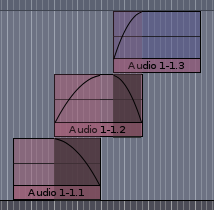
\includegraphics[scale=0.5]{stacked.png}
\end{center}
\caption{A track in stacked mode}
\label{fig:stacked}
\end{figure}

In this mode, layering is performed \emph{explicitly}.  In other words, the
user's immediate actions decide which layer a region should be put on.  When a
region move drag is started in stacked mode, the regions separate further out
vertically, to leave space between each layer, as shown in
Figure~\ref{fig:stacked-drag}.

\begin{figure}[ht]
\begin{center}
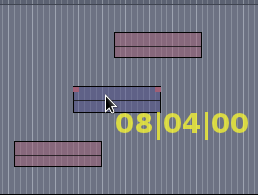
\includegraphics[scale=0.5]{stacked-drag.png}
\end{center}
\caption{A track in stacked mode during a drag}
\label{fig:stacked-drag}
\end{figure}

The region(s) being dragged can then be dropped in any location, horizontally
and vertically, and the regions will be layered accordingly.


\section{Overlaid mode}

When a track is being displayed in \emph{overlaid} mode, regions are
displayed on top of one another, like in Figure~\ref{fig:overlaid}.

\begin{figure}[ht]
\begin{center}
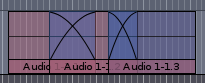
\includegraphics[scale=0.5]{overlaid.png}
\end{center}
\caption{A track in overlaid mode}
\label{fig:overlaid}
\end{figure}

In this mode, drags of regions maintain the same \emph{layer ordering}, even if the layers may
change.

\end{document}
